\ifx\wholebook\relax\else

% --------------------------------------------
% Lulu:

    \documentclass[a4paper,12pt,twoside]{../includes/ThesisStyle}

	\usepackage[T1]{fontenc} %%%key to get copy and paste for the code!
%\usepackage[utf8]{inputenc} %%% to support copy and paste with accents for frnehc stuff
\usepackage{times}
\usepackage{ifthen}
\usepackage{xspace}
\usepackage{alltt}
\usepackage{latexsym}
\usepackage{url}            
\usepackage{amssymb}
\usepackage{amsfonts}
\usepackage{amsmath}
\usepackage{stmaryrd}
\usepackage{enumerate}
\usepackage{cite}
%\usepackage[pdftex,colorlinks=true,pdfstartview=FitV,linkcolor=blue,citecolor=blue,urlcolor=blue]{hyperref}
\usepackage{xspace}
%\usepackage{graphicx}
\usepackage{subfigure}
\usepackage[scaled=0.85]{helvet}
        
        
\newcommand{\sepe}{\mbox{>>}}
\newcommand{\pack}[1]{\emph{#1}}
\newcommand{\ozo}{\textsc{oZone}\xspace}
\newcommand\currentissues{\par\smallskip\textbf{Current Issues -- }}

\newboolean{showcomments}
\setboolean{showcomments}{true}
\ifthenelse{\boolean{showcomments}}
  {\newcommand{\bnote}[2]{
	\fbox{\bfseries\sffamily\scriptsize#1}
    {\sf\small$\blacktriangleright$\textit{#2}$\blacktriangleleft$}
    % \marginpar{\fbox{\bfseries\sffamily#1}}
   }
   \newcommand{\cvsversion}{\emph{\scriptsize$-$Id: macros.tex,v 1.1.1.1 2007/02/28 13:43:36 bergel Exp $-$}}
  }
  {\newcommand{\bnote}[2]{}
   \newcommand{\cvsversion}{}
  } 


\newcommand{\here}{\bnote{***}{CONTINUE HERE}}
\newcommand{\nb}[1]{\bnote{NB}{#1}}
\newcommand{\fix}[1]{\bnote{FIX}{#1}}
%%%% add your own macros 

\newcommand{\sd}[1]{\bnote{Stef}{#1}}
\newcommand{\ja}[1]{\bnote{Jannik}{#1}}
\newcommand{\na}[1]{\bnote{Nico}{#1}}
%%% 


\newcommand{\figref}[1]{Figure~\ref{fig:#1}}
\newcommand{\figlabel}[1]{\label{fig:#1}}
\newcommand{\tabref}[1]{Table~\ref{tab:#1}}
\newcommand{\layout}[1]{#1}
\newcommand{\commented}[1]{}
\newcommand{\secref}[1]{Section \ref{sec:#1}}
\newcommand{\seclabel}[1]{\label{sec:#1}}

%\newcommand{\ct}[1]{\textsf{#1}}
\newcommand{\stCode}[1]{\textsf{#1}}
\newcommand{\stMethod}[1]{\textsf{#1}}
\newcommand{\sep}{\texttt{>>}\xspace}
\newcommand{\stAssoc}{\texttt{->}\xspace}

\newcommand{\stBar}{$\mid$}
\newcommand{\stSelector}{$\gg$}
\newcommand{\ret}{\^{}}
\newcommand{\msup}{$>$}
%\newcommand{\ret}{$\uparrow$\xspace}

\newcommand{\myparagraph}[1]{\noindent\textbf{#1.}}
\newcommand{\eg}{\emph{e.g.,}\xspace}
\newcommand{\ie}{\emph{i.e.,}\xspace}
\newcommand{\ct}[1]{{\textsf{#1}}\xspace}


\newenvironment{code}
    {\begin{alltt}\sffamily}
    {\end{alltt}\normalsize}

\newcommand{\defaultScale}{0.55}
\newcommand{\pic}[3]{
   \begin{figure}[h]
   \begin{center}
   \includegraphics[scale=\defaultScale]{#1}
   \caption{#2}
   \label{#3}
   \end{center}
   \end{figure}
}

\newcommand{\twocolumnpic}[3]{
   \begin{figure*}[!ht]
   \begin{center}
   \includegraphics[scale=\defaultScale]{#1}
   \caption{#2}
   \label{#3}
   \end{center}
   \end{figure*}}

\newcommand{\infe}{$<$}
\newcommand{\supe}{$\rightarrow$\xspace}
\newcommand{\di}{$\gg$\xspace}
\newcommand{\adhoc}{\textit{ad-hoc}\xspace}

\usepackage{url}            
\makeatletter
\def\url@leostyle{%
  \@ifundefined{selectfont}{\def\UrlFont{\sf}}{\def\UrlFont{\small\sffamily}}}
\makeatother
% Now actually use the newly defined style.
\urlstyle{leo}



	\usepackage{amsmath,amssymb}             % AMS Math
% \usepackage[french]{babel}
\usepackage[latin1]{inputenc}
\usepackage[T1]{fontenc}
\usepackage[left=1.5in,right=1.3in,top=1.1in,bottom=1.1in,includefoot,includehead,headheight=13.6pt]{geometry}
\renewcommand{\baselinestretch}{1.05}

\usepackage{multicol}

% Table of contents for each chapter

\usepackage[nottoc, notlof, notlot]{tocbibind}
\usepackage{minitoc}
\setcounter{minitocdepth}{1}
\mtcindent=15pt
% Use \minitoc where to put a table of contents

\usepackage{enumitem}

\usepackage{aecompl}

% Glossary / list of abbreviations

%\usepackage[intoc]{nomencl}
%\renewcommand{\nomname}{List of Abbreviations}
%
%\makenomenclature

% My pdf code

\usepackage[pdftex]{graphicx}
\usepackage[a4paper,pagebackref,hyperindex=true]{hyperref}

\usepackage{pgfplotstable,booktabs,colortbl}
\pgfplotsset{compat=1.8}

% Links in pdf
\usepackage{color}
\definecolor{linkcol}{rgb}{0,0,0.4} 
\definecolor{citecol}{rgb}{0.5,0,0} 

% Change this to change the informations included in the pdf file

% See hyperref documentation for information on those parameters

\hypersetup
{
bookmarksopen=true,
pdftitle="Sista: a Metacircular Architecture for Runtime Optimisation Persistence",
pdfauthor="Clement BERA", 
pdfsubject="Thesis", %subject of the document
%pdftoolbar=false, % toolbar hidden
pdfmenubar=true, %menubar shown
pdfhighlight=/O, %effect of clicking on a link
colorlinks=true, %couleurs sur les liens hypertextes
pdfpagemode=None, %aucun mode de page
pdfpagelayout=SinglePage, %ouverture en simple page
pdffitwindow=true, %pages ouvertes entierement dans toute la fenetre
linkcolor=linkcol, %couleur des liens hypertextes internes
citecolor=citecol, %couleur des liens pour les citations
urlcolor=linkcol %couleur des liens pour les url
}

% definitions.
% -------------------

\setcounter{secnumdepth}{3}
\setcounter{tocdepth}{1}

% Some useful commands and shortcut for maths:  partial derivative and stuff

\newcommand{\pd}[2]{\frac{\partial #1}{\partial #2}}
\def\abs{\operatorname{abs}}
\def\argmax{\operatornamewithlimits{arg\,max}}
\def\argmin{\operatornamewithlimits{arg\,min}}
\def\diag{\operatorname{Diag}}
\newcommand{\eqRef}[1]{(\ref{#1})}

\usepackage{rotating}                    % Sideways of figures & tables
%\usepackage{bibunits}
%\usepackage[sectionbib]{chapterbib}          % Cross-reference package (Natural BiB)
%\usepackage{natbib}                  % Put References at the end of each chapter
                                         % Do not put 'sectionbib' option here.
                                         % Sectionbib option in 'natbib' will do.
\usepackage{fancyhdr}                    % Fancy Header and Footer

% \usepackage{txfonts}                     % Public Times New Roman text & math font
  
%%% Fancy Header %%%%%%%%%%%%%%%%%%%%%%%%%%%%%%%%%%%%%%%%%%%%%%%%%%%%%%%%%%%%%%%%%%
% Fancy Header Style Options

\pagestyle{fancy}                       % Sets fancy header and footer
\fancyfoot{}                            % Delete current footer settings

%\renewcommand{\chaptermark}[1]{         % Lower Case Chapter marker style
%  \markboth{\chaptername\ \thechapter.\ #1}}{}} %

%\renewcommand{\sectionmark}[1]{         % Lower case Section marker style
%  \markright{\thesection.\ #1}}         %

\fancyhead[LE,RO]{\bfseries\thepage}    % Page number (boldface) in left on even
% pages and right on odd pages
\fancyhead[RE]{\bfseries\nouppercase{\leftmark}}      % Chapter in the right on even pages
\fancyhead[LO]{\bfseries\nouppercase{\rightmark}}     % Section in the left on odd pages

\let\headruleORIG\headrule
\renewcommand{\headrule}{\color{black} \headruleORIG}
\renewcommand{\headrulewidth}{1.0pt}
\usepackage{colortbl}
\arrayrulecolor{black}

\fancypagestyle{plain}{
  \fancyhead{}
  \fancyfoot{}
  \renewcommand{\headrulewidth}{0pt}
}

\usepackage{algorithm}
\usepackage[noend]{algorithmic}

%%% Clear Header %%%%%%%%%%%%%%%%%%%%%%%%%%%%%%%%%%%%%%%%%%%%%%%%%%%%%%%%%%%%%%%%%%
% Clear Header Style on the Last Empty Odd pages
\makeatletter

\def\cleardoublepage{\clearpage\if@twoside \ifodd\c@page\else%
  \hbox{}%
  \thispagestyle{empty}%              % Empty header styles
  \newpage%
  \if@twocolumn\hbox{}\newpage\fi\fi\fi}

\makeatother
 
%%%%%%%%%%%%%%%%%%%%%%%%%%%%%%%%%%%%%%%%%%%%%%%%%%%%%%%%%%%%%%%%%%%%%%%%%%%%%%% 
% Prints your review date and 'Draft Version' (From Josullvn, CS, CMU)
\newcommand{\reviewtimetoday}[2]{\special{!userdict begin
    /bop-hook{gsave 20 710 translate 45 rotate 0.8 setgray
      /Times-Roman findfont 12 scalefont setfont 0 0   moveto (#1) show
      0 -12 moveto (#2) show grestore}def end}}
% You can turn on or off this option.
% \reviewtimetoday{\today}{Draft Version}
%%%%%%%%%%%%%%%%%%%%%%%%%%%%%%%%%%%%%%%%%%%%%%%%%%%%%%%%%%%%%%%%%%%%%%%%%%%%%%% 

\newenvironment{maxime}[1]
{
\vspace*{0cm}
\hfill
\begin{minipage}{0.5\textwidth}%
%\rule[0.5ex]{\textwidth}{0.1mm}\\%
\hrulefill $\:$ {\bf #1}\\
%\vspace*{-0.25cm}
\it 
}%
{%

\hrulefill
\vspace*{0.5cm}%
\end{minipage}
}

\let\minitocORIG\minitoc
\renewcommand{\minitoc}{\minitocORIG \vspace{1.5em}}

\usepackage{multirow}
\usepackage{slashbox}

\newenvironment{bulletList}%
{ \begin{list}%
	{$\bullet$}%
	{\setlength{\labelwidth}{25pt}%
	 \setlength{\leftmargin}{30pt}%
	 \setlength{\itemsep}{\parsep}}}%
{ \end{list} }

\newtheorem{definition}{D�finition}
\renewcommand{\epsilon}{\varepsilon}

% centered page environment

\newenvironment{vcenterpage}
{\newpage\vspace*{\fill}\thispagestyle{empty}\renewcommand{\headrulewidth}{0pt}}
{\vspace*{\fill}}



	\graphicspath{{.}{../figures/}}
	\begin{document}
\fi

\chapter{Introduction}
\label{chap:intro}
\minitoc

\section{Context}

Object-oriented languages have been one of the most popular programming languages for the past decades. Many high-level object-oriented programming languages run on top of a virtual machine (VM)~\footnote{In the whole thesis, VM refers to a virtual machine for high-level languages, by opposition to Operating System VMs which are not discussed at all.} which provides certain advantages from running directly on the underlying hardware. 

\paragraph{Virtual machines for high-level programming languages.}
Most high-level languages pursue a strict separation between language-side and VM-side. VMs for instance provide automatic memory management or use platform independent instructions such as bytecodes. These properties allow a programming language to develop independently from the underlying hardware.

High performance VMs, such as Java HotSpot or current Javascript VMs achieve high performance through just-in-time compilation techniques: once the VM has detected that a portion of code is frequently used (called \emph{hot spot}), it recompiles it on-the-fly with speculative optimizations based on previous runs of the code. If usage patterns change and the code is not executed as previously speculated anymore, the VM dynamically deoptimizes the execution stack and resumes execution with the unoptimized code.

Such performance techniques allow object-oriented languages to greatly improve their peak performance. However, a warm-up time is required for the VM to speculate correctly about frequently used patterns. This warm-up time can be problematic for different use-cases.

Originally VMs were built in performance oriented low-level programming languages such as C. However, as the VMs were reaching higher and higher performance, the complexity of their code base increased and some VMs started to get written in higher-level languages as an attempt to control complexity. Such VMs got written either in the language run by the VM itself~\cite{Unga05b,Wimm13a,Alp99a} or in domain specific languages compiled to machine code through C~\cite{Rigo06a,Inga97a}.

\paragraph{Pharo programming language and community.}

In this thesis the focus is on a specific high-level object-oriented programming language, the Smalltalk dialect named Pharo~\cite{Blac09a}, a fork of another Smalltalk dialect named Squeak~\cite{Blac07a} made by the original Smalltalk-80 implementors. In Pharo, everything is an object, including classes, bytecoded versions of methods or processes. It is dynamically-typed and every call is a virtual call. The VM relies on a bytecode interpreter and a baseline just-in-time compiler (JIT) to gain performance. Modern Smalltalk dialects directly inherit from Smalltalk-80~\cite{Gold83a} but have evolved during the past 35 years. For example, real closures and exceptions were added.

As Pharo is evolving, its VM, the Cog VM~\cite{Mira08a}, is improving. For example, a modern memory manager was added over the past few years, improving performance and allowing the VM to use a larger amount of memory. The open-source community is now looking for new directions for VM evolutions, including better VM performance. Compared to many high performance VMs, the Pharo VM is not as efficient because it lacks an optimising JIT with speculative optimisations. The optimising JIT is usually one of the most complex part of high performance VMs. As the Pharo community has a limited amount of ressources to the maintain and evolve the VM, the idea is to design the optimising JIT in a way where open-source contributors can get involved in the maintainance and evolution tasks.

Many people in the community have high skills in object-oriented programming, especially Pharo development, while few people have skills in low-level programming such as assembly code or C. Hence, the community on average understands much more Smalltalk programs than low-level programs. Assuming one is more likely to contribute to a program one can understand, the logical choice is to design the optimising JIT in Smalltalk.

The existing production VM is written in a subset of Smalltalk~\cite{Inga97a}, called Slang, compiling through C to machine code to generate the production VM. Hence, two directions could be taken to write the optimising JIT in Smalltalk. On the one hand, the optimising JIT could be written in Slang, the existing subset of Smalltalk, like the existing VM. On the other hand, it could be written in the complete Smalltalk language, with a design similar to the metacircular VMs~\cite{Unga05b,Wimm13a,Alp99a}. Compared to C and assembly code, Slang tends to abstract away machine concepts to leverage the development experience closer to Smalltalk. However, an important part of the community does not contribute to the VM because its code-base is not available in the base system (it has been compiled to an executable ahead of time) and because they do not entirely understand the remaining low-level aspects. For this reason, writting the optimising JIT in the complete Smalltalk language seems to be the best option.

%Removed
%However, Slang was designed primarily for a pure interpreter-based VM. Its first version included the minimum set of features required to have a simple interpreter and memory manager running. Then, to increase performance, the interpreter was improved and a baseline JIT was added. Both new components were more complex than the existing code. As they were added by customer demands requiring short-term delivery, multiple features got incrementally added in Slang, each time making sure the VM could still compile but without entirely rethinking the semantics or re-working the Slang-to-C compiler. As a result, Slang is now quite complex and the addition of new features is now difficult. In fact, the current VM maintainers believe that the VM complexity has reached the limit that Slang can handle without an important redesign of its features. Adding an optimising JIT, more complex than existing code, did not seem to be the right thing to do.

%Removed
%The community considered falling into a modern trend which consists of reusing existing VM for other programming languages to run Pharo to drastically decrease the ressources spent in VM maintenance. For example, the RPython toolchain(CITE) and the Truffle framework(CITE) allows teams to easily build high-performance VM with a limited investment of ressources. This was not the direction taken for four main reasons:
%\begin{itemize}
%	\item Doing so would weaken the VM knowledge in the Pharo community as there will be no VM maintainer in the it (all VM maintainers would be in the used framework community).
%	\item Few people in the community would have the skills to understand and contribute to such a VM due to the language barrier, as the common skills in the community are Smalltalk skills, and none of those frameworks are written in Smalltalk.
%	\item Part of the system would potentially not be understood by anyone understanding both Pharo and the VM, leading to uncommon crashes that no one can understand or solve.
%	\item Pharo have exotic features that may not be supported by such framework. Even if such features are supported, they may be supported without the required performance or they may not be supported in the future as the Pharo community has no major influence on such framework communities.
%\end{itemize}
	
To conclude, the Pharo community is looking for better VM performance and the next step to improve the performance of the existing VM is to add an optimising JIT. To attract open-source contributors from the community, the optimising JIT has to be written in Smalltalk.

\paragraph{Existing design.}

A first optimising JIT design emerged in the early 2000s for another Smalltalk VM, a precursor of the current Pharo VM. The design is the convergence of multiple ideas to ease the development of the optimising JIT, to ensure that the maintainance and evolution cost of the resulting implementation is going to be reasonnable and to attract contributors from the community.

As most of the community has high skills in Smalltalk but little skills in low-level programming, one of the idea is to split the optimising JIT in two parts, as shown on figure \ref{fig:ExistingDesign}. The first part, the high level part, may deal with Smalltalk-specific optimisation and compiles to well-specified platform independent instructions. The second part, the low-level part, can translate such instructions into machine code, performing machine-specific optimisations.

\begin{figure}[h!]
    \begin{center}
        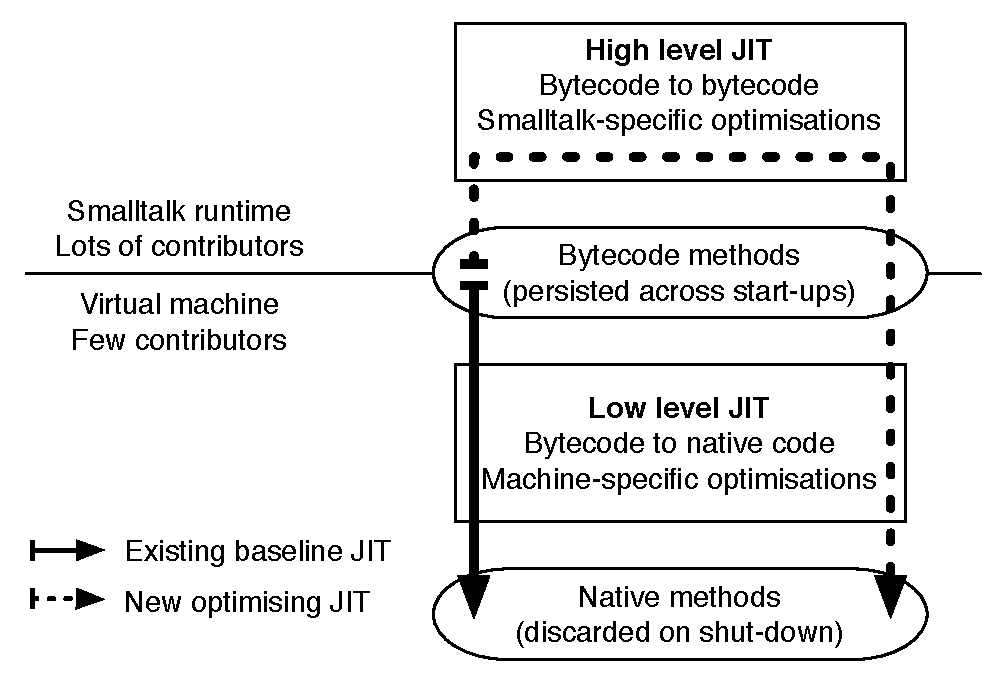
\includegraphics[width=0.8\linewidth]{ExistingDesign}
        \caption{JIT compilation model design}
        \label{fig:ExistingDesign}
    \end{center}
\end{figure}

The high-level part can be written in Smalltalk entirely, in a metacircular style. This way, members of the Pharo community can contribute to a project in Smalltalk doing Smalltalk-specific optimisations, improving performance while staying away from low-level details and machine-specific optimisations. 

After discussing with other VM implementors, it seems that language-specific optimisations (in our case Smalltalk-specific optimisations) are more important than machine-specific optimisations for performance. As the community has a smaller number of low-level contributors, another idea is then to reuse the existing baseline JIT, already present in the VM, as the low-level part. Reusing the existing baseline JIT as a back-end for the optimising JIT means there is only one code-base to maintain and evolve for all the low-level aspects of both JITs. To ease the implementation of this design, the interface between the two parts of the optimising JIT was conceived as an extended bytecode set (the existing bytecode set with the addition of new operations used only by optimised code). This way, the existing baseline JIT already supporting the existing bytecode set would "just" need to be slightly extended to support the new operations.

Lastly, the high-level part of the JIT is generating platform-independent optimised bytecode methods. Bytecode methods can already be persisted across multiple start-ups. The last idea is therefore to persist optimised code, in the form of optimised bytecode methods, to avoid most of the warm-up time present in many modern VMs.

Some aspects of the design were considered, analyzed and discussed very carefully by part of the Smalltalk community, making the design attractive and interesting. However, the overall design was incomplete so it was unclear how multiple parts of the system would work. 

The thesis started from this proposal, in an attempt to complete the design and propose an implementation. Multiple aspects of the design are different from existing VMs. The advantages and issues of these differences are discussed in the thesis.

\section{Problem}

During the thesis, the main research direction was the following:
\emph{How to build an optimising JIT for Pharo, written in Pharo itself, running in the same runtime than the optimised application on top of the existing runtime environment ?} 

%Metacircular pb
By design, the optimising compiler has to run in the same runtime as the running application. As the optimising JIT is written in the optimised language, it may be able to optimise its own code. This behavior may lead to strange interactions between multiple parts of the runtime, leading to performance loss or crashes. The Graal compiler~\cite{Dubo13c} has a similar design to what we are trying to build. It can run on top of the Java hotspot VM as an alternative optimising JIT. In this case, as Java is multithreaded, it runs in the same runtime than the running application but in different native threads. In Graal though, the development team avoids most of these problems by keeping part of the deoptimisation logic and the stack analysis to determine what method to optimise in the hotspot VM and not in the Java runtime. 

%Persistance
As the attempt to implement the proposal was started to execute code, we analysed the interaction between optimising JITs and Smalltalk-style \emph{snapshots}. In Smalltalk, a normal programmer regularly takes a snapshot, a memory dump of all the existing objects, to save the running system state. The Smalltalk VM normally starts-up by resuming execution from a snapshot, restoring all the object states and resuming all running green threads. Each green thread has its own execution stack, which may refer to optimised code. In most existing VMs, the optimised code is not persisted across multiple start-ups, making difficult the persistance of green threads unless all stack frames present in their execution stack are deoptimised. With the bytecode to bytecode optimisation design, the persistance of running green threads, including the persistance of optimised code they refer to, may be possible across multiple start-ups.

%VM-language interface
%Based on the existing design, the optimising JIT was implemented in the thesis mostly as a bytecode-to-bytecode optimiser. In this context, an expressive interface between the high-level part of the optimising JIT, doing language-specific optimisations in Smalltalk and the low-level part, doing machine-specific optimisations and written in Slang had to be designed. To ease the development and get results quicker, the interface was designed as an extended bytecode set. This interface is good enough to show performance improvements and very convenient to demonstrate the persistance of optimised code across start-ups. A different interface, more specific for the optimising JIT can be considered to bypass some limitations and may be more expressive. In the Graal compiler, which is as far as we know the project with the closest design, machine code is generated from the language-side optimiser hence the interface between the VM and the language had to be extended very differently.

\paragraph{Research subproblems.}The thesis focuses on 
two %three 
aspects in the context of the main problem:
\begin{itemize}
	\item \emph{Metacircular optimising JIT:} In the context of an optimising JIT written in the single-threaded language it optimises, can the JIT optimise its own code at runtime and if so, under which constraints ?
	\item \emph{Runtime state persistance:} How to persist the runtime state across multiple VM start-ups, including the running green threads and the optimised code ?
	%\item \emph{Virtual function instruction set:} How to design an expressive instruction set between to have the high-level part and the low-level part of the optimising JIT, both completely independent and written in different programming languages, communcating efficiently ?
\end{itemize}

\section{Contributions}

The main contributions of this thesis are, in the context of the Pharo programming language:
\begin{itemize}
	\item An optimising JIT running on top of the existing production virtual-machine, showing improved performance in execution time.
	\item An alternative bytecode set solving multiple existing encoding limitations.
	\item A language extension: each object can now be marked as read-only.
	\item An alternative implementation of closures, both allowing simplifications in existing code and enabling new optimisation possibilities.
\end{itemize}

\section{Overview}

The thesis present the \emph{Sista architecture} (\textbf{S}peculative \textbf{I}nlining \textbf{S}mall\textbf{T}alk \textbf{A}rchitecture). The architecture features an optimising JIT written in Smalltalk running on top of the existing Pharo VM. The optimising JIT is running in the same runtime than the optimised application. Sista is able to persist the runtime state of the program across multiple start-ups. %The communication between the rest of the VM and the optimising JIT is done through a minimal interface.

\section{Terminology}

\paragraph{Functions and frames.} In the thesis we use the term \emph{function} to discuss executable code, which corresponds in practice to a method or a closure. More specifically, we distinguish \emph{virtual functions}, or v-functions, which can be executed by a virtual machine (in our case, bytecode version of functions) and \emph{native function}, or n-function, the native code version of a function executed by a specific processor. 

We discuss VMs using an hybrid runtime where v-functions can be executed either through a v-function interpreter or by executing the corresponding n-function generated by a JIT from the v-function. On the one hand, we call \emph{virtual frame} or v-frame a stack frame used by the v-function interpreter. On the other hand, we call \emph{native frame} or n-frame a stack frame used by the execution of a n-function. V-frames have typically a machine-independent representation and all the values used by the execution stored inside the frame, while n-frames may have a machine-dependent representation and may have some values in registers.

%Moved to state-of-the-art.
\paragraph{Tiered architecture.} One of the most common high-performance VM architecture is the tiered architecture: the first few executions of v-functions are performed by an interpreter and subsequent executions falls into the JIT infrastructure, composed of multiple tiers. Each JIT tier requires more time to compile the v-function to n-function than the previous tier, but the resulting n-function is more efficient. In most VMs, there are two JIT compiler tiers. The first tier is called the \emph{baseline JIT}. It translates quickly v-functions to n-functions with a limited number of optimisations. The baseline JIT typically generates n-functions with inline caches to collect type information. The other tier is called the \emph{optimising JIT}. It translates v-functions to highly optimised n-functions with speculative optimisations, based on the runtime information collected on n-functions generated by the baseline JIT.

%Should move this to Architecture.
\paragraph{Sista.} \emph{Sista} is the named of the architecture detailled in the thesis. As the architecture has notable differences from the standard tiered architecture, the two runtime compilers are not really a baseline JIT and an optimising JIT. We call them by their project name in the thesis. The first runtime compiler is called \emph{Scorch} and compiles v-functions to optimised v-functions using speculative optimisations. Scorch is written in plain Smalltalk. The second runtime compiler is called \emph{Cogit} and compiles v-functions to n-functions. Cogit can be used alone as the baseline JIT, or as a back-end for Scorch. In the later case, the pair of Scorch and Cogit forms an optimising JIT. Cogit is written in a restrictive Smalltalk compiled ahead-of-time to an executable as part of the VM. 

In this context, both v-functions and n-functions can have an optimised version. We therefore used the term v-function to discuss all v-functions (optimised or not), and specify optimised v-function and non optimised v-function when needed. Similarly, for frames, we say v-frame to discuss v-frames in general, and specify optimised v-frame and non optimised v-frame when discussing a v-frame respectively representing the execution state of an optimised v-function or a non optimised v-function. The same terminology is used with native (\emph{n-}) than with virtual (\emph{v-}).

Both runtime compilers can deoptimise stack frames. Cogit can deoptimise any n-frame to a single v-frame. 
%Cogit also provides proxies to introspect a n-frame as a v-frame, though certain operations such as instruction pointer mutation do not work with proxies but require deoptimisation from a n-frame to a v-frame. 
Scorch can deoptimise an optimised v-frame to multiple non optimised v-frames. 

\section{Outline}

\begin{itemize}
	\item Chapter \ref{chap:stateOfTheArt} presents existing production and research virtual machines relevant in the context of the thesis. 
	\item Chapter \ref{chap:existing} detail the existing Pharo runtime as Sista is built on top of it.
	\item Chapter \ref{chap:architecture} details the Sista architecture and chapter \ref{chap:runtimeEvolution} discuss the evolutions done on the Pharo runtime to have the Sista architecture working.
	\item Chapters \ref{chap:metacircular} and \ref{chap:persistance} 
	%and \ref{chap:interface} 
	discuss the architecture in the context of the two subproblems of the thesis. 
	\item Chapter \ref{chap:validation} evaluates the Sista architecture by comparing the performance of the runtime in multiple contexts.
\end{itemize}



\ifx\wholebook\relax\else
    \end{document}
\fi